%----------------------------------------------------------------------------------------
%	PACKAGES AND OTHER DOCUMENT CONFIGURATIONS
%----------------------------------------------------------------------------------------

\documentclass[a4paper, 11pt]{article} % Font size (can be 10pt, 11pt or 12pt) and paper size (remove a4paper for US letter paper)

\usepackage[protrusion=true,expansion=true]{microtype} % Better typography
\usepackage{graphicx} % Required for including pictures
\usepackage{wrapfig} % Allows in-line images

\usepackage{mathpazo} % Use the Palatino font
\usepackage[T1]{fontenc} % Required for accented characters
\linespread{1.05} % Change line spacing here, Palatino benefits from a slight increase by default

\usepackage{natbib}
\usepackage{attrib}
\usepackage{pgf-pie}

\tolerance=1
\emergencystretch=\maxdimen
\hyphenpenalty=10000
\hbadness=10000

% CUSTOM
\usepackage{url}
\usepackage{subfig}
\usepackage{amsfonts}
\usepackage{booktabs}
\usepackage{siunitx}
\usepackage[page]{appendix}
\usepackage{dcolumn}
\usepackage{rotating}


\makeatletter
\renewcommand\@biblabel[1]{\textbf{#1.}} % Change the square brackets for each bibliography item from '[1]' to '1.'
\renewcommand{\@listI}{\itemsep=0pt} % Reduce the space between items in the itemize and enumerate environments and the bibliography

\renewcommand{\maketitle}{ % Customize the title - do not edit title and author name here, see the TITLE block below
\begin{flushright} % Right align
{\LARGE\@title} % Increase the font size of the title
\vspace{50pt} % Some vertical space between the title and author name

{\large\@author} % Author name
\\\ \today % Date

\vspace{40pt} % Some vertical space between the author block and abstract
\end{flushright}
}

%TC:incbib % Count words

%----------------------------------------------------------------------------------------
%	TITLE
%----------------------------------------------------------------------------------------
%%TC:ignore
\title{\textbf{Analysis of Microdata: Tanzania}\\ % Title
Policy Evaluation and Applied Statistics } % Subtitle

\author{\textsc{Roman Küpper} % Author
\\{\textit{MAS Development and Cooperation NADEL ETHZ 20-22}}} % Institution

\date{\today} % Date

%----------------------------------------------------------------------------------------

%----------------------------------------------------------------------------------------
%	CUSTOM
%----------------------------------------------------------------------------------------
\usepackage{multirow}
\usepackage[colorlinks,citecolor=blue,urlcolor=black,bookmarks=false,hypertexnames=true]{hyperref} 



\begin{document}

\maketitle % Print the title section


%----------------------------------------------------------------------------------------
%	ESSAY BODY
%----------------------------------------------------------------------------------------

\section{Introduction}
% Not sure if i want to keep the subsections in the introduction -> maybe better to merge them in to one
While stunting and mortality for children under five has declined in most countries over the last decades, they are still important issues for countries in sub-Saharan Africa \cite{Nshimyiryo2019Dec}. The reduction of child mortality is also indirectly linked to a reduced fertility due to the higher chances of a child's survival \cite{uddin2009}. Furthermore they are and have been an important topic in development for the last decades. The reduction of child mortality is the stated aim of Goal 4 of the Millennium Development Goals (MDGs) and the health of children is mentioned in several of the Sustainable Development Goals (SDGs). To successfully lower the stunting and child-mortality rates, it is vastly important to understand the underlying causes. The following article will analyse data from the Demographic and Health Survey (DHS) for Tanzania to identify country-specific factors that determine if a child is in risk of being stunted or prone to die below the age of five. The study will focus mainly on the effects of per-household income and examine if income is a necessary and sufficient condition for improvements in child health. [TODO: Short overview of dataset, variables used, method, findings and conclusion]

\subsection*{Tanzania}
The situation of Tanzanian children in regard to stunting and under-five mortality has improved over the last three decades. The prevalence for stunting could be decreased from 50\% in the 1990s to 34\% in the year 2015 \cite{UNI18}. The same applies for the under-five mortality rate. The sex-specific under-five mortality rate dropped from 171 to 54 per 1000 births for boys and from 159 to 47 per 1000 births for girls from 1990 to 2019 \cite{UN20}. But despite improvements in recent year, stunting and child mortality in Tanzania are still an ongoing issue in the country. 


\subsection*{Other literature}
Previous research have shown a number of different factors that have an influence on stunting and under-five mortality. Those include the age and sex of the child and various factors concerning the mothers health and education. But also socio-economic factors like the household wealth are mentioned. The factors mentioned in the literature differ for stunting and under-five mortality. Unfinished listings for both, stunting and under-five mortality, can be found in the according tables in Appendix \ref{sec:appendixa} and Appendix \ref{sec:appendix_tab_mortality}. The tables in the appendix also show how the factors are matched with the variables in our dataset. Factors often mentioned as related to stunting are child age, sex of child, birth weight, birth size, mothers health, mothers education, mothers age, mothers BMI, breastfeeding, wealth of household, social inequality, source of drinking water, sanitation and place of residence \cite{Akombi2017Aug}\cite{UNI18}. \\

Some of the factors related with stunting are also mentioned as factors for under-five mortality which is not surprising since the most severe forms of stunting often lead to death. Literature lists sex of child, birth order, malnutrition, vaccinations, access to postnatal care, mothers age, education, breastfeeding, place of delivery, household wealth, place of residence , source of drinking water and sanitation as some of the most important factors for under-five mortality according to \cite{Ettarh2012Mar}\cite{Who2020Sep} and \cite{UNICEF2006}. 


\section{Methods} \label{sec:methods}
\subsection*{Data sources}

In order to analyse the relationship between income and under-5 mortality and stunting rate a dataset based on the Demographic and Health Surveys (DHS) \cite{DHS20} by ICF International is used. The dataset contains panel data of Tanzanian households for the years 2005, 2010 and 2015. The dataset consists of 24,198 observations for 15,273 households.

\begin{table}[!htbp]
  \small
  \centering
  \setlength\tabcolsep{2pt}
    \scalebox{0.8}{
  \centerline{
    \begin{tabular}{lllll}
    \hline
     &  \textbf{2005} & \textbf{2010} & \textbf{2015} & \textbf{Overall} \\ 
     &  \textbf{(N=7727)} & \textbf{(N=7303)} & \textbf{(N=9168)} & \textbf{(N=24198)} \\ \hline
    \textbf{Stunting} & & & &  \\		
    no	& 3775 (48.9\%) &	3772 (51.7\%) &	5736 (62.6\%) &	13283 (54.9\%) \\
    yes	& 2854 (36.9\%) &	2581 (35.3\%) &	2501 (27.3\%) &	7936 (32.8\%) \\
    missing &	1098 (14.2\%) &	950 (13.0\%) &	931 (10.2\%) &	2979 (12.3\%) \\ \hline
    \textbf{Under-5 years mortality} & & & &  \\
    no	& 7303 (94.5\%) &	7050 (96.5\%) &	8928 (97.4\%) &	23281 (96.2\%) \\
    yes	& 424 (5.5\%) &	253 (3.5\%) &	240 (2.6\%) &	917 (3.8\%) \\ \hline
    \textbf{Under-1 year mortality} & & & &  \\						
    no &	1664 (21.5\%) &	1541 (21.1\%) &	1887 (20.6\%) & 5092 (21.0\%) \\
    yes &	282 (3.6\%) &	167 (2.3\%) &	144 (1.6\%) & 593 (2.5\%) \\
    missing &	5781 (74.8\%) &	5595 (76.6\%) &	7137 (77.8\%) & 18513 (76.5\%) \\ \hline
    \textbf{Under-1 month mortality} & & & &  \\						
    no &	69 (0.9\%) &	68 (0.9\%) &	82 (0.9\%) & 219 (0.9\%) \\
    missing &	7658 (99.1\%) &	7235 (99.1\%) &	9086 (99.1\%) & 23979 (99.1\%) \\ \hline
    \textbf{Household income} & & & &  \\						
    Mean (SD) &	66.6 (56.5) &	78.0 (60.1) &	82.2 (68.1) &	76.0 (62.5) \\
    Median [Min, Max] &	48.2 [6.43, 485] & 60.3 [13.2, 438] & 62.7 [11.2, 426] & 60.3 [6.43, 485] \\ \hline
    \textbf{Place of residence} & & & &  \\						
    rural &	6383 (82.6\%) &	5918 (81.0\%) &	7034 (76.7\%) &	19335 (79.9\%) \\
    urban &	1344 (17.4\%) &	1385 (19.0\%) &	2134 (23.3\%) &	4863 (20.1\%) \\ \hline
    \textbf{Child age (months)} & & & &  \\						
    Mean (SD) &	28.2 (17.6) &	29.1 (17.6) &	29.0 (17.5) & 28.8 (17.6) \\
    Median [Min, Max] &	27.0 [0, 60.0] &	29.0 [0, 60.0] & 28.0 [0, 60.0]	& 28.0 [0, 60.0] \\ \hline
    \textbf{Child sex} & & & &  \\						
    male &	3846 (49.8\%) &	3626 (49.7\%) &	4590 (50.1\%) & 12062 (49.8\%) \\
    female &	3881 (50.2\%) &	3677 (50.3\%) &	4578 (49.9\%) & 12136 (50.2\%) \\ \hline
    \textbf{Water: improved} & & & &  \\						
    no &	4048 (52.4\%) &	3822 (52.3\%) &	3999 (43.6\%) & 11869 (49.0\%) \\
    yes &	3679 (47.6\%) &	3481 (47.7\%) &	5169 (56.4\%) & 12329 (51.0\%) \\ \hline
    \textbf{Sanitation: improved} & & & &  \\						
    no &	7328 (94.8\%) &	5841 (80.0\%) &	3068 (33.5\%) & 16237 (67.1\%) \\
    yes &	399 (5.2\%) &	1462 (20.0\%) &	6100 (66.5\%) & 7961 (32.9\%) \\ \hline
    \textbf{Mothers age (years)} & & & &  \\						
    Mean (SD) &	29.1 (6.80) &	29.7 (6.98) &	29.5 (7.13) & 29.4 (6.99) \\
    Median [Min, Max] &	28.0 [15.0, 49.0] & 29.0 [15.0, 49.0] &	29.0 [15.0, 49.0] &	29.0 [15.0, 49.0] \\ \hline
    \textbf{Mothers age (years) at first birth} & & & &  \\						
    Mean (SD) &	19.0 (3.10) &	19.2 (3.12) &	19.4 (3.34) & 19.2 (3.20) \\
    Median [Min, Max] &	19.0 [10.0, 35.0] & 19.0 [10.0, 41.0] &	19.0 [10.0, 46.0] &	19.0 [10.0, 46.0] \\ \hline
    \textbf{Mothers total children} & & & &  \\						
    Mean (SD) &	4.18 (2.55) &	4.26 (2.52) &	4.06 (2.57) & 4.16 (2.55) \\
    Median [Min, Max] &	4.00 [1.00, 14.0] & 4.00 [1.00, 15.0] &	3.00 [1.00, 17.0] &	4.00 [1.00, 17.0] \\ \hline
    \textbf{Mothers breastfeeding status} & & & &  \\						
    no &	3017 (39.0\%) &	2926 (40.1\%) &	3789 (41.3\%) & 9732 (40.2\%) \\
    yes &	4710 (61.0\%) &	4377 (59.9\%) &	5379 (58.7\%) & 14466 (59.8\%) \\ \hline
    \textbf{Mother received prenatal care} & & & &  \\						
    no &	4230 (54.7\%) &	3344 (45.8\%) &	8705 (94.9\%) & 16279 (67.3\%) \\
    yes &	3497 (45.3\%) &	3959 (54.2\%) &	463 (5.1\%) & 7919 (32.7\%) \\ \hline
    \textbf{Mother received medical assistance} & & & &  \\						
    no	& 4584 (59.3\%) &	3878 (53.1\%) &	8323 (90.8\%) &	16785 (69.4\%) \\
    yes	& 3143 (40.7\%) &	3425 (46.9\%) &	845 (9.2\%) &	7413 (30.6\%) \\ \hline
    \textbf{Mother education} & & & &  \\						
    noedu &	3390 (43.9\%) &	2986 (40.9\%) &	3208 (35.0\%) & 9584 (39.6\%) \\
    primary &	4235 (54.8\%) &	4225 (57.9\%) &	5052 (55.1\%) & 13512 (55.8\%) \\
    secondary &	102 (1.3\%) &	92 (1.3\%) &	908 (9.9\%) & 1102 (4.6\%) \\ \hline
    \end{tabular}
  }}
  \caption{General descriptive statistics of baseline characteristics of the study population}
  \label{table:descriptive_gen}
\end{table}

\subsection*{Research Strategy}

The aim of this research is to provide a better understanding of the effectiveness of income on under-5-mortality and stunting. For this reason multiple regression models are built to estimate the influence of different independent variables on the two dependent variables (stunting and under-5-mortality). In a first step, only the influence of income on stunting and under-5-mortality IS examined. The formula for the traditional ordinary least squares model (\ref{eqn:simple_regression}) is shown below:

\begin{equation}
 Y_i = \beta_0 + \beta_1 X_i + u_i
 \label{eqn:simple_regression}
\end{equation}

Next, the models are adjusted for survey-year time-fixed effects (\ref{eqn:time_fixed_regression}) with the formula:

\begin{equation}
Y_{it} = \beta_0 + \beta_1 X_{it} + \delta_T BT_t + u_{it}
 \label{eqn:time_fixed_regression}
\end{equation}

The models are then further improved by adding other potentially meaningful variables (\ref{eqn:time_fixed_multiple_regression}) to further reduce the error term. The formula for the multiple regression with regard to time-fixed effects is:

\begin{equation}
Y_{it} = \beta_0 + \beta_1 X_{it} + \delta_2 B2_t + \cdots + \delta_T BT_t + u_{it}
 \label{eqn:time_fixed_multiple_regression}
\end{equation}

Starting from the simple ordinary least square (OLS) regression the model will be further enhanced by controlling for additional variables and time fixed effects. 

\subsection*{Data sources and procedures}
To provide a better understanding of the dataset, some descriptive statistics of the most interesting variables is shown in this section. A tabular overview can be found in
 table \ref{table:descriptive_gen} and table \ref{table:descriptive_mo}, with table \ref{table:descriptive_gen} focusing on general characteristic of the dataset and shows some information on the distribution of our dependent variables stunting and under-five mortality and table \ref{table:descriptive_mo} focusing on a set of variables containing information on the mother which are important determinant of a children's health and well-being. Some information is further presented in graphs to allow a better visual interpretation. \\
 
 The dataset contains information from surveys in 2005, 2010 and 2015. The whole number of children included in the dataset it 24,198. The number of children has declined slightly from the first survey in 2005 with 7.727 observations in 2005 to 7,303 in 2010 but has then inclined to 9,168 in 2015. \\


\begin{figure}[h]
    \centering
    \subfloat[\centering Under-five mortality]{{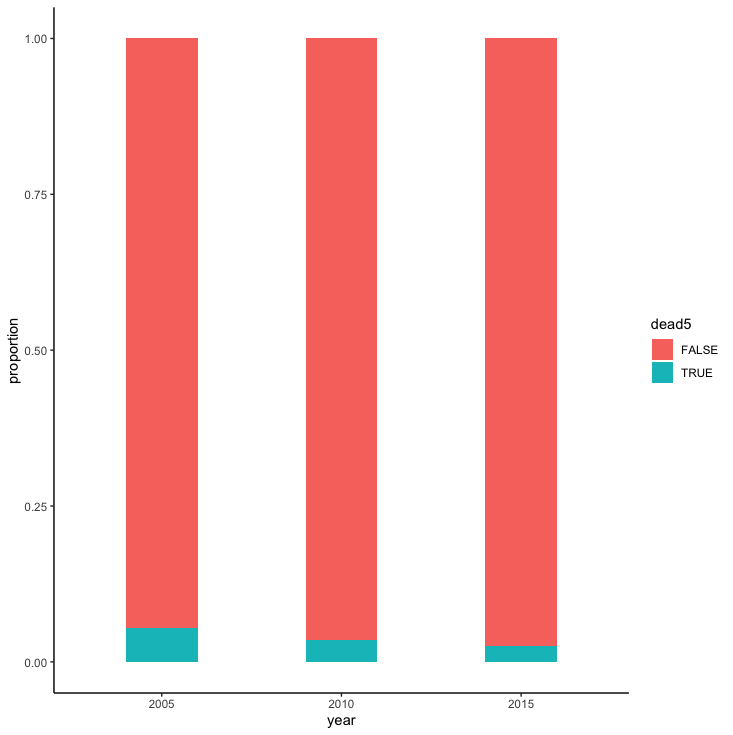
\includegraphics[width=5cm]{figures/dead5_proportion} }}%
    \qquad
    \subfloat[\centering Stunting]{{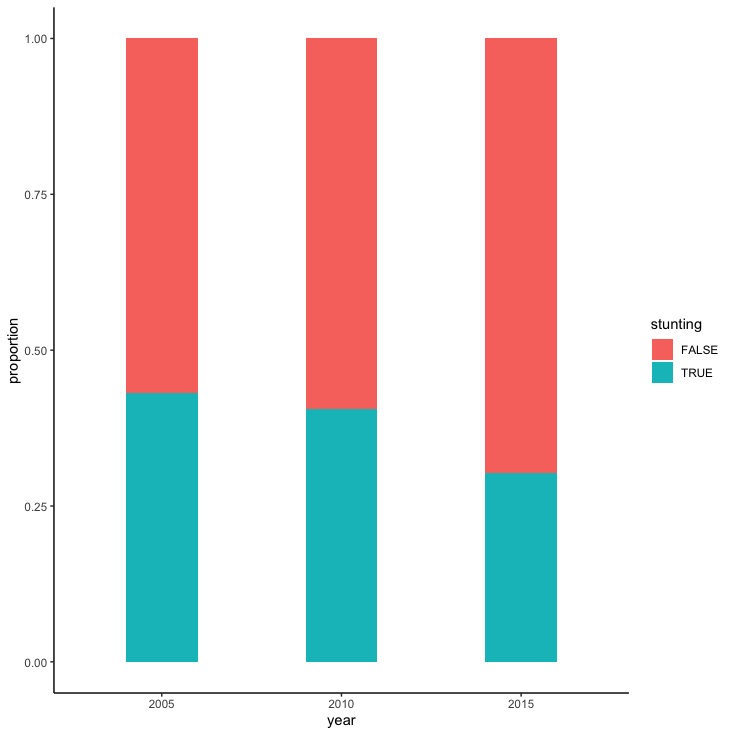
\includegraphics[width=5cm]{figures/stunting_proportion} }}%
    \caption{Proportions of children that are stunted or have died under the age of fiver over time}%
    \label{fig:stunting_dead5_proportion}%
\end{figure}

\subsection*{Outcomes}

The share of children that are stunted as well as the share of children dying under five has declined through the three time periods. A visualization of this trend can be seen in figure \ref{fig:stunting_dead5_proportion} which shows the proportions of both variables over time. The figure also shows that while child-mortality has been vastly reduced, stunting is still a widely spread issue in Tanzania.

\begin{figure}[!h]
    \centering
    \subfloat[\centering Access to improved water]{{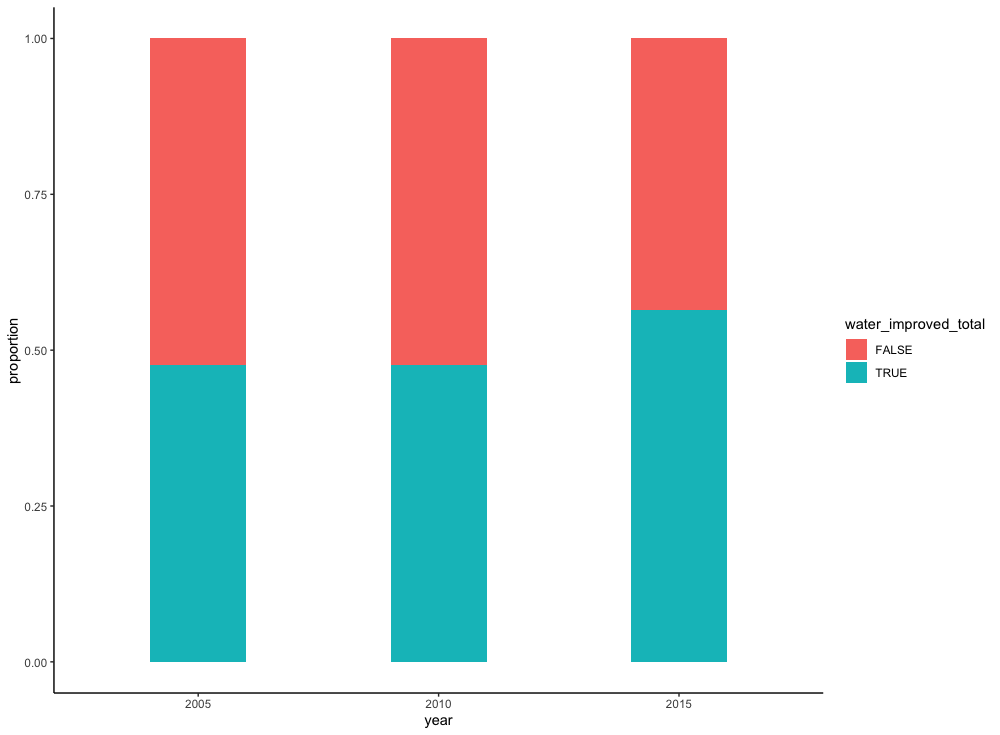
\includegraphics[width=5cm]{figures/water_improved_proportion} }}%
    \qquad
    \subfloat[\centering Access to improved sanitation]{{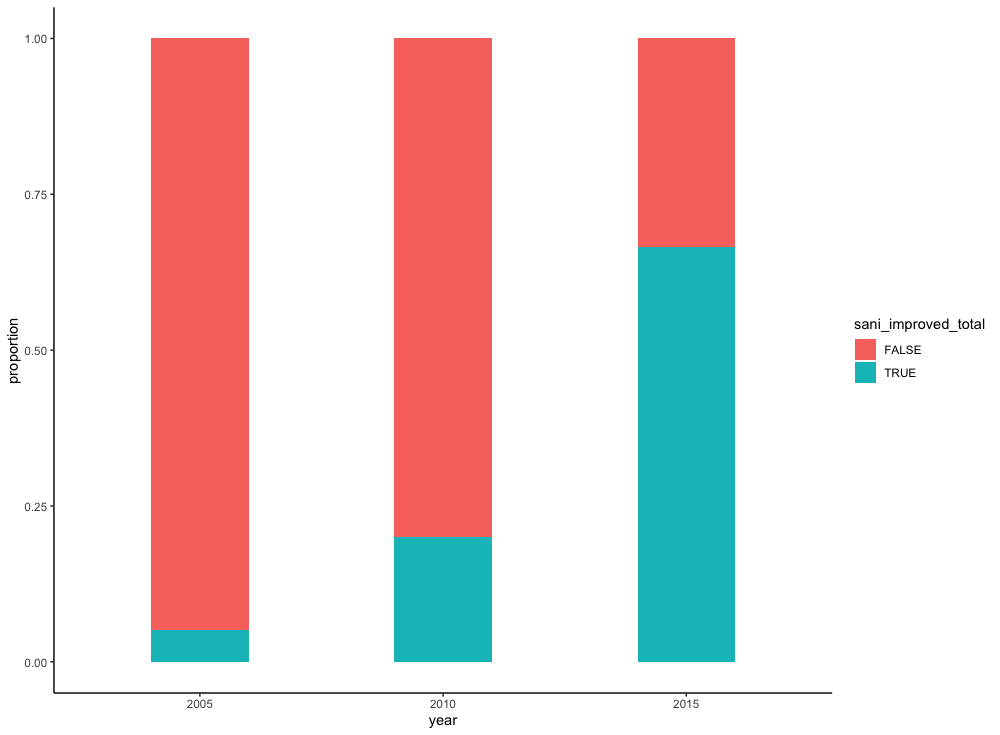
\includegraphics[width=5cm]{figures/sanitation_improved_proportion} }}%
    \caption{Proportions of children with access to improved water and sanitation over time}%
    \label{fig:water_sanitation_proportion}%
\end{figure}

The access to clean water sources and improved sanitation are also substantively important variables for the well-being of children. If they are lacking they can cause life-threatening diseases like diarrhoea that are under suspicion to cause up to 50\% of all child malnourishment \cite{UNI18}. The share of children with access to improved water and sanitation is shown in figure \ref{fig:water_sanitation_proportion}. The figures for improved water as well as improved sanitation show an upward trend with the share of improved sanitation (see figure \ref{fig:water_sanitation_proportion}(b)) having climbed more rapidly than the share of access to improved water (see figure \ref{fig:water_sanitation_proportion}(a)). The trend towards better water and sanitation is in line with the Tanzanian governments vision for a more healthy society from 2007 \cite{Health2016Dec}.


Another often quoted factor for the well-being of children is their mothers education. The dataset includes information on three different variables for education. Namely primary, secondary and no education. The interpretation of the data is somewhat difficult. Some of the observations specify that a mother has both primary and no education at the same time. When this data is interpreted as "the mother has started but not finished her primary education", the corresponding barplot is shown in figure (\ref{fig:education_proportion})(a). 

\begin{figure}[h!]
    \centering
    \subfloat[\centering Lower education if in doubt]{{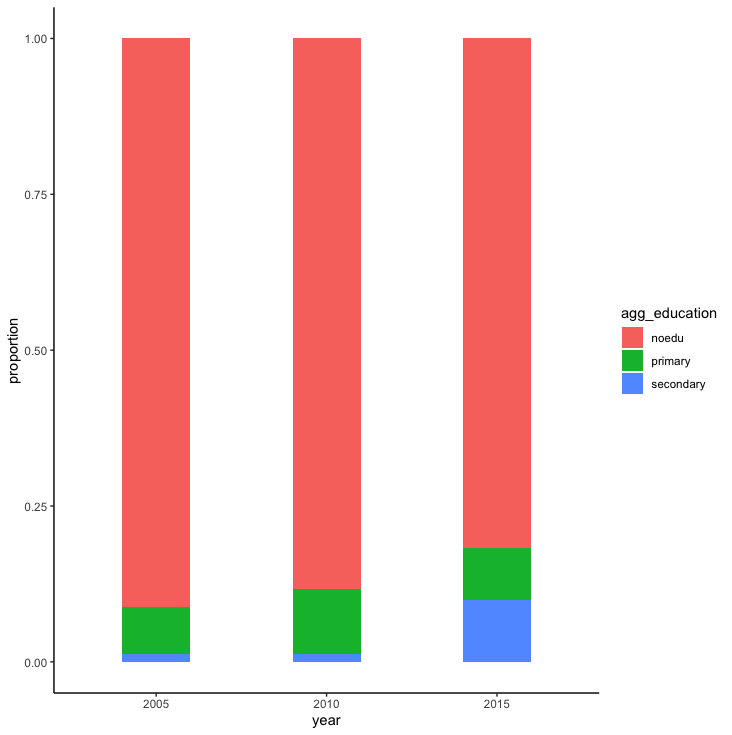
\includegraphics[width=5cm]{figures/aggregated_education_indoubt_lower} }}%
    \qquad
    \subfloat[\centering Higher education if in doubt]{{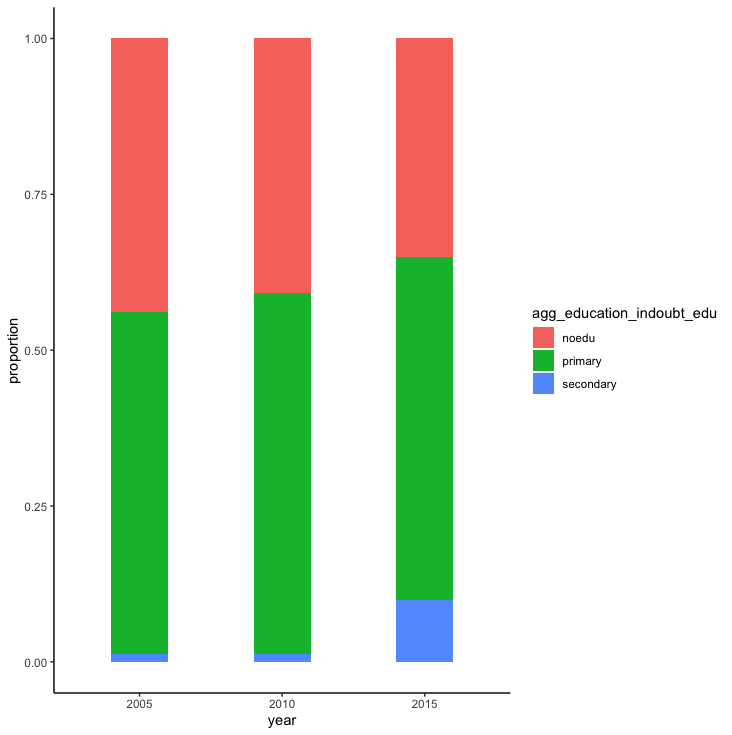
\includegraphics[width=5cm]{figures/aggregated_education_indoubt_higher} }}%
    \caption{Mothers education levels over time}%
    \label{fig:education_proportion}%
\end{figure}

But when looking at other studies on the distribution of primary, secondary on no-education in Tanzania, the share of uneducated women seems to be too high. If the ambiguous values are interpreted as "the education is not finished yet, but will be"\footnote{When an observation has "mo\_noedu == 1" and "mo\_primary== 1" the variables are aggregated to  to "education = primary".}, our data is more in line with other studies \cite{SAM08}. The graphic representation of this can be found in figure (\ref{fig:education_proportion})(b).  





\section{Results}

\begin{sidewaystable}[!htbp] \centering 
  \caption{Regressions Using Demographic and Health Surveys} 
  \label{table:regression_models} 
  \scalebox{0.75}{
\begin{tabular}{@{\extracolsep{5pt}}lD{.}{.}{-5} D{.}{.}{-5} D{.}{.}{-5} D{.}{.}{-5} D{.}{.}{-5} D{.}{.}{-5} } 
\\[-1.8ex]\hline 
\hline \\[-1.8ex] 
 & \multicolumn{6}{c}{\textit{Dependent variable:}} \\ 
\cline{2-7} 
\\[-1.8ex] & \multicolumn{3}{c}{stunting} & \multicolumn{3}{c}{dead5} \\ 
 & \multicolumn{1}{c}{(I)} & \multicolumn{1}{c}{(II)} & \multicolumn{1}{c}{(III)} & \multicolumn{1}{c}{(IV)} & \multicolumn{1}{c}{(V)} & \multicolumn{1}{c}{(VI)} \\ 
\\[-1.8ex] & \multicolumn{1}{c}{OLS} & \multicolumn{1}{c}{Fixed effects} & \multicolumn{1}{c}{Full} & \multicolumn{1}{c}{OLS} & \multicolumn{1}{c}{OLS fixed effects} & \multicolumn{1}{c}{Full}\\ 
\hline \\[-1.8ex] 
 log\_y & -0.10287^{***} & -0.09724^{***} & -0.06590^{***} & -0.00832^{***} & -0.00632^{***} & -0.00354 \\ 
  & (0.00431) & (0.00433) & (0.00568) & (0.00162) & (0.00161) & (0.00222) \\ 
  as.factor(urban)urban &  &  & -0.04095^{***} &  &  & 0.00569^{*} \\ 
  &  &  & (0.00891) &  &  & (0.00341) \\ 
  c\_age &  &  & 0.00288^{***} &  &  &  \\ 
  &  &  & (0.00020) &  &  &  \\ 
  c\_sex &  &  & -0.05025^{***} &  &  &  \\ 
  &  &  & (0.00645) &  &  &  \\ 
  c\_first &  &  &  &  &  & 0.02076^{***} \\ 
  &  &  &  &  &  & (0.00370) \\ 
  mo\_assistance &  &  &  &  &  & -0.00630^{**} \\ 
  &  &  &  &  &  & (0.00314) \\ 
  mo\_age\_birth &  &  & -0.00137^{***} &  &  & 0.00180^{***} \\ 
  &  &  & (0.00048) &  &  & (0.00023) \\ 
  as.factor(mo\_breastfeeeding)yes &  &  & -0.04524^{***} &  &  & -0.02895^{***} \\ 
  &  &  & (0.00757) &  &  & (0.00267) \\ 
  mo\_primary &  &  & -0.03265^{***} &  &  & -0.00395 \\ 
  &  &  & (0.00707) &  &  & (0.00272) \\ 
  mo\_secondary &  &  & -0.06947^{***} &  &  & -0.01304^{***} \\ 
  &  &  & (0.01342) &  &  & (0.00442) \\ 
  water\_improved\_total &  &  & -0.02413^{***} &  &  & -0.00982^{***} \\ 
  &  &  & (0.00710) &  &  & (0.00273) \\ 
  sani\_improved\_total &  &  & -0.02135^{**} &  &  & -0.00636^{**} \\ 
  &  &  & (0.00908) &  &  & (0.00317) \\ 
  Constant & 0.79150^{***} & 0.81154^{***} & 0.78864^{***} & 0.07170^{***} & 0.07966^{***} & 0.04294^{***} \\ 
  & (0.01817) & (0.01828) & (0.02868) & (0.00689) & (0.00710) & (0.01069) \\ 
 \hline \\[-1.8ex] 
Observations & \multicolumn{1}{c}{21,219} & \multicolumn{1}{c}{21,219} & \multicolumn{1}{c}{21,219} & \multicolumn{1}{c}{24,198} & \multicolumn{1}{c}{24,198} & \multicolumn{1}{c}{24,198} \\ 
R$^{2}$ & \multicolumn{1}{c}{0.02397} & \multicolumn{1}{c}{0.03486} & \multicolumn{1}{c}{0.05857} & \multicolumn{1}{c}{0.00102} & \multicolumn{1}{c}{0.00462} & \multicolumn{1}{c}{0.01457} \\ 
Adjusted R$^{2}$ & \multicolumn{1}{c}{0.02392} & \multicolumn{1}{c}{0.03472} & \multicolumn{1}{c}{0.05803} & \multicolumn{1}{c}{0.00098} & \multicolumn{1}{c}{0.00449} & \multicolumn{1}{c}{0.01408} \\ 
\hline 
\hline \\[-1.8ex] 
\textit{Note:}  & \multicolumn{6}{r}{$^{*}$p$<$0.1; $^{**}$p$<$0.05; $^{***}$p$<$0.01} \\ 
\end{tabular}
}
\end{sidewaystable}

The variables included in the models are chosen based on the available dataset, the existing literature and intuition. To further get insights on variables with a significant impact on both outcome variables, a series of correlation matrices was created. The final matrices can be found in Appendix \ref{fig:corrmatrix_stunting} and Appendix \ref{fig:corrmatrix_dead5}. The circles in each matrix show how each set of variables on X- and Y-axis are correlated. The color of a circle determines how strong the correlation is and if it is positive or negative correlated. Colour intensity and the size of the circles are proportional to the correlation coefficients. The analysis of the two correlation matrices already gives a first impression on the effects of the different independent variables on our outcome variables. While we won't go into detail with with interpretation of the matrices, it is interesting to see, how correlated some of the variables are. The findings from the visual analysis will go into the creation of our regression models presented in this section. \\

In a first step of the statistical analysis, an ordinary least squares regression model is chosen to estimate the effects of income-changes on the binary outcome variables stunting and under-five mortality. To allow for a better interpretation, the natural logarithm of a households income (log\_y) is chosen. The overall strategy is to judge the influence of a per household income change on a child's probability to be stunted or to die under the age of five while controlling for time-fixed effects and other influential variables. The control variables differ between stunting and under-five mortality. Not the whole dataset contains information on stunting. Observations that have missing values on stunting are omitted for the regression model that is built for stunting. This leads to a reduction of observations for the models (I-III) compared to the models (IV-VI) from 24,198 to 21,219. \\

The findings are listed in table \ref{table:regression_models} (I-III) for stunting and (IV-VI) for under-five mortality. In column (I) for stunting and column (IV) for under-five mortality we can see the results of the most simple OLS regression. As our outcome variables are binary (stunting / not stunting and dead under-five and alive under-five) and our independent variable is the natural logarithm of the household income the effect is estimated based on percentage changes in income. For stunting this means, that an additional percent of income would lead to a by 0.1 percentage point decreased probability of a child being stunted. For under-five mortality this effect is a lot smaller and the additional percent of income would only lead to a decrease of 0.008 percentage points. Both effects are significant to a significance level of 5\%. \\

In section \ref{sec:methods} it was shown that stunting and under-five mortality rates have been declined over time. Since it cannot be certain that all explaining variables have been included in our model it it important to control for time-fixed effects. They are included to control for the fact that we can expect the number of stunting and dying children to be declining based on factors we cannot control for that are changing over time. If those time-fixed effects are included the effect of additional income is shrinking slightly. This could be due to long-term results of the vision for a more healthy society in Tanzania or better access to health related articles, a better understanding of the matter or other effects that aren't included in the model or where no data is available. But even with time-fixed effects included both effects, while being small, are still significant. \\

The final models are shown in (III) and (VI) of table \ref{table:regression_models}. For stunting, the additional variables on the place of residence, child age, child sex, mothers age at birth, mother is breastfeeding, mothers education, water and sanitation are included. With this variables included, the effect that is explained by additional income further decreases to 0.007 percentage points. All of the variables mentioned have a significant effect, but the effect of sanitation is only significant to a lower significance level of 10\%. In total 0.003 percentage points of the original effect could be explained by time fixed effects and other variables. But even with all those variables included, household income still has the second highest impact on the probability of a child being stunted. Other important factors are if the mother has a secondary education, the child's sex, if the mother is breastfeeding and place of residence (urban).  \\

For under-five mortality the additional variables on the place of residence, first-born child, mother got assistance, mother got care, mothers age at birth, mother is breastfeeding, mothers education, water and sanitation are included. With this additional variables included the effect of income further declines and is not significant anymore. The two most variables with the largest effect on under-five mortality are if the mother is breastfeeding, if the child is the first-born and if the mother got secondary education. Water and sanitation also have measurable effects on under-five mortality. Since both of those correlate with income, it could be that the higher income already explains a large share of the income effects. Also the comparatively high effect of a child being the first-born could be interpreted as a lacking knowledge or experience of a mother that could lead to a higher chance of the child to die. But to answer our initial question, it seems as if income is not a sufficient condition for a smaller risk of a child to die under the age of five.


\section{Discussion}
There are some limitation to the presented model, since some of variables suggested to have an impact by previous research, could not be included. This could lead us to tend to evaluate the impact of income as too large. Also it has to be kept in mind that some of the variables used in the models (III) and (VI) are correlated between themselves as shown in the correlation matrices in Appendix \ref{sec:appendixc} and \ref{sec:appendixd}. An enhanced model should therefore explicitly test for multicollinearity by including a variance inflation factor (VIF). 

Would be interesting to look at some variables that we couldn't add to the model due to missing data: dead0, dead1, mo\_noedu


%----------------------------------------------------------------------------------------
% BIBLIOGRAPHY
%----------------------------------------------------------------------------------------
\newpage
\bibliographystyle{plain}
\bibliography{main.bib}

%----------------------------------------------------------------------------------------

%----------------------------------------------------------------------------------------
% APPENDIX
%----------------------------------------------------------------------------------------
\newpage
\section*{Appendices}
\appendix
\section{Household income distribution over time} \label{sec:appendix_household_dist}
\begin{figure}[h!]
    \centering
    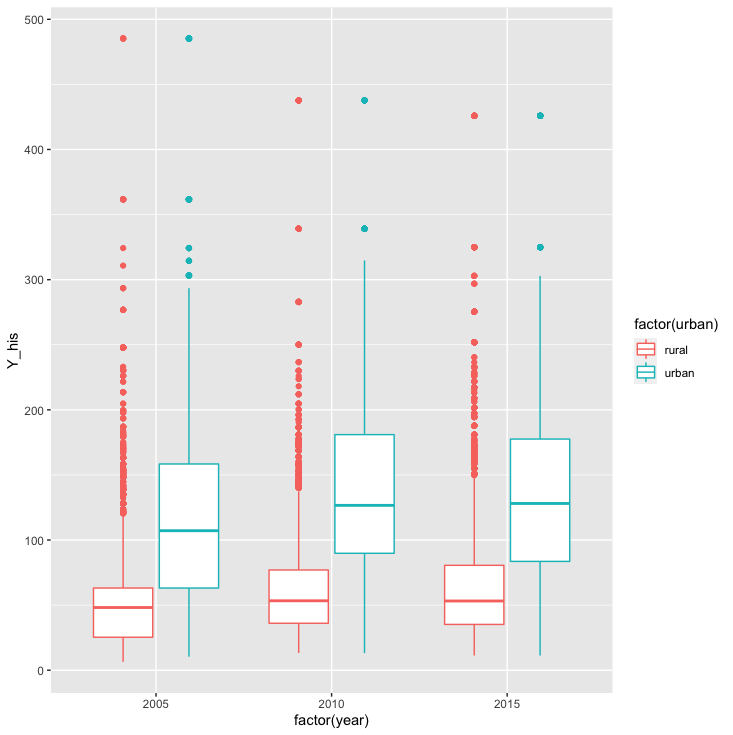
\includegraphics[scale=0.5]{figures/income_over_time} 
    \caption{Y\_his over time}
    \label{fig:income_over_time}
\end{figure}

\newpage
\section{Factors and variables for stunting} \label{sec:appendix_tab_stunting}
\begin{table}[h!]
\begin{tabular}{@{}lll@{}}
\toprule
\# & \textbf{Factors} & \textbf{Corresponding variable} \\ \midrule
1 & Childs age & c\_age \\
2 & Sex of child & c\_sex  \\
3 & Birth weight & -  \\
4 & Birth size & - \\ \midrule

5 & Mothers health & - \\
6 & Mothers education & mo\_noedu, mo\_primary, mo\_secondary \\
7 & Mothers age  & mo\_age\_birth \\
8 & Mothers BMI & - \\
9 & Breastfeeding & mo\_breastfeeding \\ \midrule

10 & Wealth of household & Y\_his  \\
11 & Social inequality & income\_quintile \\
12 & Source of drinking water & water\_improved\_total  \\
13 & Sanitation &  sani\_improved\_total  \\
14 & Place of residence & urban  \\ \bottomrule
\end{tabular}
    \caption{Factors associated with childhood stunting, wasting and underweight. Sources: \cite{Akombi2017Aug} \cite{UNI18}}
    \label{table:stunting}
\end{table}

\newpage
\section{Factors and variables for under-five mortality} \label{sec:appendix_tab_mortality}
\begin{table}[h!]
\begin{tabular}{@{}lll@{}}
\toprule
\# & \textbf{Factors} & \textbf{Corresponding variable} \\ \midrule
1 & Sex of child & c\_sex  \\
2 & Birth order & c\_first  \\ 
3 & Malnutrition & - \\ 
4 & Vaccinations & - \\ \midrule

5 & Access to postnatal care & mo\_assistance \\
6 & Mothers age & mo\_age\_birth \\
7 & Education & mo\_noedu, mo\_primary, mo\_secondary \\
8 & Breastfeeding & mo\_breastfeeding \\
9 & Place of delivery & - \\ \midrule

10 & Household wealth & Y\_his \\
11 & Place of residence  & urban \\ 
12 & Source of drinking water & water\_improved\_total  \\
13 & Sanitation &  sani\_improved\_total  \\ \bottomrule
\end{tabular}
    \caption{Factors associated with under-five mortality. Sources: \cite{Ettarh2012Mar}\cite{Who2020Sep}} \cite{UNICEF2006}
    \label{table:dead5}
\end{table}


\newpage
\section{Correlation-matrix for stunting} \label{sec:appendixc}
\begin{figure}[h!]
    \centering
    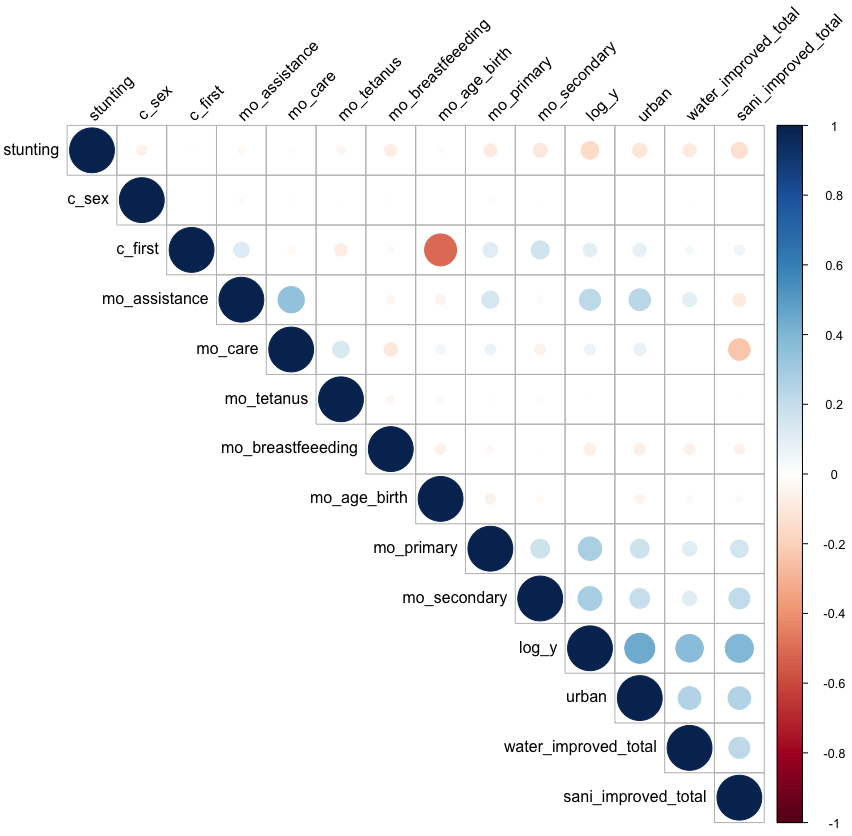
\includegraphics[scale=0.45]{figures/corrmatrix_stunting_4} 
    \caption{Correlation-matrix that should help to find variables that have a significant effect on stunting.}
    \label{fig:corrmatrix_stunting}
\end{figure}


\newpage
\section{Correlation-matrix for under-five mortality} \label{sec:appendixd}
\begin{figure}[h!]
    \centering
    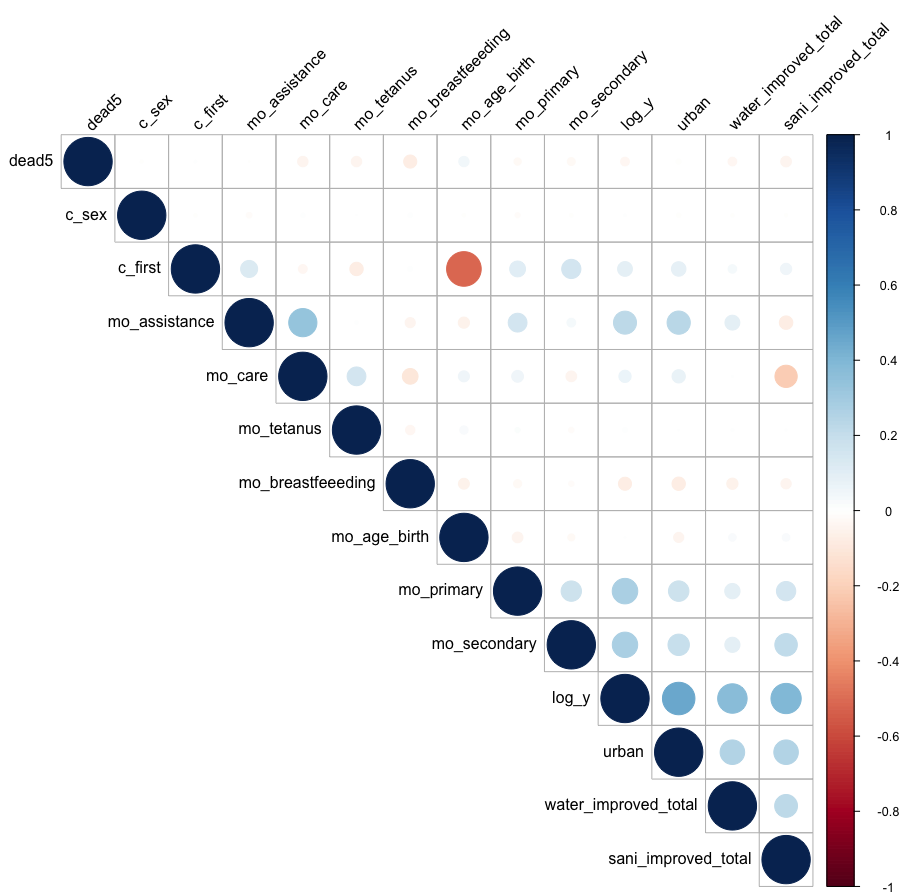
\includegraphics[scale=0.45]{figures/corrmatrix_dead5_4} 
    \caption{Correlation-matrix that should help to find variables that have a significant effect on under-five mortality.}
    \label{fig:corrmatrix_dead5}
\end{figure}

%----------------------------------------------------------------------------------------

\end{document}